\documentclass[11pt]{article}

\usepackage[utf8]{inputenc}
\usepackage[T1]{fontenc}
\usepackage{lmodern}
\usepackage[margin=1in]{geometry}
\usepackage{amsmath,amssymb,amsthm}
\usepackage{booktabs}
\usepackage{graphicx}
\usepackage{enumitem}
\usepackage{xcolor}
\usepackage[hidelinks]{hyperref}

% Figures are bundled in ./figures/ so the paper is self-contained (zip-safe);
% ../Code/figures/ is kept as a fallback when building inside the repo.
\graphicspath{{figures/}{./figures/}{../Code/figures/}}

\setlength{\parindent}{0pt}
\setlength{\parskip}{0.55em}
\setlength{\emergencystretch}{3em}

\newcommand{\Sig}{\Sigma}
\newcommand{\Sighat}{\hat\Sigma}
\newcommand{\R}{\mathbb{R}}
\newcommand{\E}{\mathbb{E}}
\newcommand{\tr}{\operatorname{tr}}
\newcommand{\diag}{\operatorname{diag}}
\newcommand{\one}{\mathbf{1}}
\newcommand{\w}{\mathbf{w}}
\newcommand{\vv}{\mathbf{v}}
\newcommand{\bb}{\mathbf{b}}
\newcommand{\uu}{\mathbf{u}}
\newcommand{\M}{M(\w)}
\newcommand{\lammin}{\lambda_{\min}}
\newcommand{\lammax}{\lambda_{\max}}

\newtheorem{proposition}{Proposition}
\newtheorem{lemma}{Lemma}
\newtheorem{corollary}{Corollary}

\title{\bfseries A Design-Optimality Regularizer for Portfolio Selection: 
  A/D/E-Optimality as Structured Shrinkage}
\author{Sukhdeep Singh and Saumen Mandal \\ \\
Department of Statistics, University of Manitoba, Winnipeg, MB, R3T 2N2, Canada}
%\author{Sukhdeep Singh\thanks{Undergraduate Research Assistantship. Advisor: Prof.\ Saumen Mandal.}}
%\date{\today}
\date{}

\begin{document}
\maketitle

\begin{abstract}
Global minimum-variance (GMV) portfolios are notoriously unstable: they invert a
noisy covariance estimate, so small estimation errors are amplified into large,
concentrated, high-turnover weights. We propose a unified, convex portfolio
optimizer that adds to the Markowitz risk objective a family of penalties
using the theory of \emph{optimal experimental design}. Reading the portfolio weights
as a design measure over a factor regression, we define a weight-dependent
information matrix 
%$\M=B^\top\diag(\w)B$ 
and regularize the portfolio through the
classical A-, D-, and E-optimality criteria. The three criteria
correspond to distinct, economically interpretable goals---minimum average
factor-estimation variance (A), balanced factor coverage / diversification (D),
and worst-case robustness (E)---and each is convex, admits closed-form
gradients, and preserves the two canonical special cases (plain GMV and
ridge-GMV) exactly. On synthetic data every criterion moves its own target
quantity monotonically in the predicted direction; in a high-dimensional simulation, 
%($N/T\to1$) 
the design penalties keep the weights stable where the
sample-covariance Markowitz portfolio collapses; and on a real data application of universe of US
sector ETFs the design-regularized portfolio cuts turnover roughly tenfold
versus sample Markowitz while quadrupling effective breadth, at comparable
risk-adjusted return. Our methodology unifies ridge/shrinkage regularization,
diversification, and robust portfolio selection under a single design-theoretic
lens.
\end{abstract}

\vspace{0.2cm}

{\bf Keywords}: 
Optimal design, portfolio optimizer, Markowitz risk, design measure, information matrix, shrinkage regularization, diversification, robust portfolio selection.

% =====================================================================
\section{Introduction and motivation}
% =====================================================================
Markowitz mean--variance selection \cite{markowitz1952} is the foundation of
quantitative portfolio construction, but in its pure form it is fragile. The
global minimum-variance (GMV) portfolio, 
\[
  \w_{\mathrm{GMV}}=\frac{\Sig^{-1}\one}{\one^\top\Sig^{-1}\one},
\]
depends on the \emph{inverse} of the covariance matrix, and in practice $\Sig$ is
replaced by a sample estimate $\Sighat$ formed from a finite window of returns.
Estimation error in $\Sighat$ is amplified by the inversion: the smallest
eigenvalues of $\Sighat$ (the least-well-estimated directions) dominate
$\Sighat^{-1}$, producing weights that are extreme, concentrated in a few
assets, unstable across rebalances, and expensive to trade
\cite{brittenjones1999}. When the number of assets $N$ approaches the number of
observations $T$, $\Sighat$ becomes ill-conditioned or singular and the problem
is acute.

The standard responses regularize the estimate or the weights. Ridge / diagonal
loading replaces $\Sighat$ with $\Sighat+\lambda I$; Ledoit--Wolf shrinkage
pulls $\Sighat$ toward a structured target \cite{ledoitwolf2004}; norm
constraints on $\w$ stabilize the solution \cite{demiguel2009norm, man17}; and the naive
$1/N$ portfolio, which uses \emph{no} estimate at all, is a famously hard
benchmark to beat out of sample \cite{demiguel2009}. Each of these is, in effect,
a statement about the \emph{spectrum} of the risk model: do not let the optimizer
exploit near-flat directions that are really just noise.

\emph{Optimal experimental design} is the branch of statistics that formalizes
exactly this concern. A design chooses how to allocate observations so that the
resulting parameter estimates are as precise as possible, and it does so by
scalarizing an information matrix through the classical A-, D-, and E-optimality
criteria \cite{atk07, fed72, bergerwong, pukelsheim2006}. The central observation of this paper
is that portfolio weights on the budget simplex play the same role as a design
measure, and that the A/D/E criteria give a principled, interpretable, and
\emph{convex} family of regularizers---each targeting a different, named failure
mode of the raw GMV portfolio.

Asset holdings and design measures share a simplex constraint. This analogy motivates exposure coverage for A and E, but does not establish that holdings generate statistical information. For D, we adopt the classical log-weight barrier that the original full-rank construction implies exactly. This distinguishes the exposure-sensitive A/E terms from an asset-level diversification control.

The optimal design perspective is useful because portfolio variance alone does not describe how holdings are distributed across economically relevant directions. For example, in the universe of US sector exchange-traded funds considered in Section 6, two allocations can have similar estimated variance yet place very different weight on funds with distinct exposure profiles. An A-optimality penalty discourages allocations with large \emph{average inverse coverage} across specified factor directions; the classical D-optimality log-weight barrier discourages nearly zero holdings across the eligible funds; and an E-optimality penalty protects the \emph{least covered} factor direction. 
%These are complementary choices about the structure of an allocation rather than guarantees of lower realized risk. 
The sector-fund example makes their roles concrete: the criteria let a portfolio designer examine whether apparent risk reduction comes at the expense of narrow holdings or weak coverage of a direction specified in advance.

\paragraph{Contribution.} We (i) formulate a single convex optimizer that unifies
mean--variance risk, ridge regularization, and A/D/E design penalties over a
composable constraint set; (ii) give the design terms a genuine
\emph{factor-regression} interpretation, so the information matrix
$\M=B^\top\diag(\w)B$ measures the precision with which the portfolio identifies
common factors, and the target parameter is the vector of factor premia;
(iii) establish convexity, closed-form gradients, optimality conditions, uniqueness, and
the two exact reductions (GMV and ridge-GMV) that serve as unit tests; and
(iv) evaluate the method on synthetic data, in a high-dimensional simulation, and
on a real sector-ETF universe, reporting both its wins and its honest
trade-offs.

% =====================================================================
\section{Portfolio problem and design-based regularization}
% =====================================================================
\subsection{The portfolio problem}
For $N$ assets with return vector $r$ and covariance $\Sig=\operatorname{Cov}(r)$,
the long-only budget-constrained GMV problem is
\[
  \min_{\w}\ \w^\top\Sig\,\w
  \quad\text{s.t.}\quad \one^\top\w=1,\ \ \w\ge0,
\]
optionally with box caps $\ell_i\le w_i\le u_i$ and group (sector) caps
$\sum_{i\in g}w_i\le c_g$. We work with an estimate $\Sighat$ supplied by any
covariance estimator (sample, Ledoit--Wolf, OAS, EWMA).

\subsection{From a design measure to portfolio weights}
In optimal design, a design is a probability measure $p=(p_1,\dots,p_J)$ on a set
of \emph{design points} (regressor vectors) $\{\vv_1,\dots,\vv_J\}$, and the
Fisher information matrix of the associated regression is
\[
  M(p)=\sum_{j=1}^{J}p_j\,\vv_j\vv_j^\top .
\]
The decision vector $p$ lives on the probability simplex $\{p\ge0,\ \one^\top p=1\}$
---which is exactly the long-only budget set of the portfolio problem. This is the
first half of the bridge: \textbf{portfolio weights $\w$ are a design measure}.
Reading $\w$ in place of $p$ and choosing per-asset vectors $\vv_i$ gives a
\emph{weight-dependent information matrix}
\begin{equation}
  \M=\sum_{i=1}^{N} w_i\,\vv_i\vv_i^\top=V\diag(\w)V^\top,
  \qquad V=[\vv_1,\dots,\vv_N]^\top ,
  \label{eq:infomat}
\end{equation}
which is \emph{linear} in $\w$ and symmetric positive semidefinite on the simplex. 

The symmetry follows from its definition, and, the positive semidefiniteness 
of the appropriate quadratic form is easy to verify: 
\begin{eqnarray*}
\mathbf{x}^{\top} \M \mathbf{x} 
= \mathbf{x}^{\top}E_{w}[\mathbf{v}\,\mathbf{v}^{\top}]\mathbf{x} 
      %\nonumber\\
= E_{w}[\mathbf{x}^{\top}\mathbf{v}\,\mathbf{v}^{\top}\mathbf{x}] 
      %\nonumber\\
= E_{w}[(\mathbf{x}^{\top}\mathbf{v})^{2}] \,\, \geq 0. \nonumber
\end{eqnarray*}



\subsection{What is $\vv_i$? A factor-regression interpretation}
\label{sec:vi}
The design object \eqref{eq:infomat} is only meaningful once we say what the
regression is. We adopt a \textbf{factor model} for returns,
\begin{equation}
  r_t = B\,f_t + \varepsilon_t,
  \qquad B\in\R^{N\times K},\ \
  \E[f_t]=\mu_f,\ \operatorname{Cov}(\varepsilon_t)=D,
  \label{eq:factor}
\end{equation}
where the $i$-th row $\bb_i^\top$ of the loading matrix $B$ is asset $i$'s vector
of exposures to $K$ common factors, $f_t$ is the vector of factor returns, and
$\varepsilon_t$ is idiosyncratic noise. This is the workhorse structure of asset
pricing \cite{fama1993} and the natural home for a regression reading of the
design criteria.

Set the design points equal to the \textbf{factor loadings}, $\vv_i=\bb_i$. Then
the target parameter is $\theta=\mu_f$, the vector of \textbf{factor premia}, and
the weight-dependent information matrix is
\begin{equation}
  \M=\sum_{i=1}^{N} w_i\,\bb_i\bb_i^\top=B^\top\diag(\w)B .
  \label{eq:factorinfo}
\end{equation}
Interpretation: If we regress portfolio-level information about the factors on
the assets we hold, $\M$ is (up to scale) the Fisher information the portfolio
carries about the factor premia, and its inverse $\M^{-1}$ is the covariance of
the corresponding estimates. The A/D/E criteria of $\M$ therefore control
\emph{how precisely, and how evenly, the portfolio identifies the common
factors}. This answers the ``what is $\vv_i$'' question directly: the $\vv_i$ are
genuine regressors (factor exposures), not an abstract device.

\paragraph{Two concrete choices of $V$.}
\begin{itemize}[leftmargin=1.4em,itemsep=0.2em]
  \item \emph{Explicit factors.} $V=B$ from an observable factor model
    (e.g.\ Fama--French) or from statistical factors (the top-$K$ principal
    components of $\Sighat$). Here the criteria act on the $K\times K$ factor
    information matrix and have the economic reading above.
  \item \emph{Precision metric (implicit factors).} Taking $V=\Sighat^{-1/2}$
    (normalized so $\tfrac1N\tr(VV^\top)=1$) makes $\M=\Sighat^{-1/2}\diag(\w)\Sighat^{-1/2}$
    a full-rank whitened information matrix; this is the limiting case in which the
    ``factors'' are the principal directions of the risk model itself. It ties the
    regularizer to the covariance with no external data and is the default used in
    our current experiments.
\end{itemize}

$M(w)$ aggregates weighted outer products of asset exposures. It measures \emph{coverage of specified exposure directions}, not the variance of $w^\top r$ and not automatically the Fisher information for factor premia. In the standard factor return model $r_t=Bf_t+\varepsilon_t$, historical observations of each asset are available independently of which assets are held today. Merely changing $w$ leaves the likelihood of the historical observations unchanged. A literal information reading requires a separate experiment: for example, an analyst purchases $n_i\propto w_i$ independent signals $y_{ij}=v_i^\top\theta+\epsilon_{ij}$ of common precision, in which case the information per unit signal budget is $\sum_iw_i v_iv_i^\top/\sigma^2$. Alternatively, unequal signal precisions replace $v_i$ by $v_i/\sigma_i$. This data-acquisition interpretation is optional and is not claimed for ordinary portfolio holdings.

A weighted factor \emph{exposure} matrix may also be confused with portfolio factor exposure $V^\top w$. These are different: $M(w)$ is a second moment of the individual asset exposure vectors and does not ensure that the \emph{net} exposure $V^\top w$ is close to any desired target. Net exposure must be addressed with separate linear constraints or penalties.

%\paragraph{One honest caveat.} 
The information matrix $\M$ is \emph{linear} in $\w$, whereas portfolio
variance $\w^\top\Sig\w$ is \emph{quadratic} in $\w$. The design--finance bridge
is therefore exact at the level of \emph{matrices and criteria} and heuristic at
the level of the weight vector; we use the design criteria as regularizers added
to the (quadratic) risk objective, not as a replacement for it.

% =====================================================================
\section{A-, D-, and E-optimality regularized portfolios}
% =====================================================================
\subsection{The unified objective}
The regularized portfolio solves
\begin{equation}
  \min_{\w} F(w) \; = 
  \underbrace{\w^\top\Sighat\,\w}_{\text{risk}}
  +\underbrace{\lambda_2\lVert\w\rVert_2^2}_{\text{ridge}}
  +\underbrace{\gamma_A\,\tr\!\big(\M^{-1}\big)}_{\text{A: average variance}}
  -\underbrace{\gamma_D\textstyle\sum_i\log w_i}_{\text{D: diversification}}
  -\underbrace{\gamma_E\,\lammin\!\big(\M\big)}_{\text{E: robustness}}
  \label{eq:objective}
\end{equation}
subject to $\one^\top\w=1$, $\ell_i\le w_i\le u_i$, and $\sum_{i\in g}w_i\le c_g$,
with all penalty strengths $\lambda_2,\gamma_A,\gamma_D,\gamma_E\ge0$. Setting all
penalties to zero recovers GMV; turning on only the ridge recovers ridge-GMV
(Section~\ref{sec:reductions}). Each of the three design terms summarizes the
information matrix $\M$ by a single number \cite{bergerwong}; we derive and
interpret them next.

\subsection{The three criteria and their economic meaning}
\paragraph{A-optimality (average factor variance).} A-optimality minimizes the
average variance of the parameter estimates, $\tr(\M^{-1})$. With
$\M=V\diag(\w)V^\top$ and $B_{\!*}=(V^\top V)^{-1}$,
\[
  \tr(\M^{-1})=\sum_{i=1}^{N}\frac{(B_{\!*})_{ii}}{w_i},
\]
a weighted inverse barrier that diverges as any $w_i\to0$ and, alone under the
budget, is minimized at $w_i\propto\sqrt{(B_{\!*})_{ii}}$. Economically, A pushes
the portfolio toward the allocation that estimates the \emph{average} factor
premium most precisely; it is a mean-variance-of-estimation criterion,
complementary to the volume (D) and worst-case (E) criteria. It is a
\emph{regularizer}, not a risk minimizer---minimizing average estimation variance
is not the same as minimizing portfolio variance, a trade-off we document
empirically.

\paragraph{D-optimality (diversification).} D-optimality maximizes $\log\det\M$.
For full-rank $V$,
\[
  \log\det\M=\log\det(VV^\top)+\sum_{i=1}^{N}\log w_i,
\]
so up to a constant, maximizing $\log\det\M$ is maximizing $\sum_i\log w_i$: the
classical \textbf{log-barrier}. Added to the minimization as
$-\gamma_D\sum_i\log w_i$, it is maximized at $\w=\tfrac1N\one$, pushes mass off
the boundary, and is the spectral face of diversification. (Note the constant
$\log\det(VV^\top)$ drops out, which is precisely why a term built on the raw
$\Sighat$ rather than on $\M$ would be inert in $\w$.)

\paragraph{E-optimality (robustness).} E-optimality maximizes the smallest
eigenvalue $\lammin(\M)$, defending the least-informed direction. As a
variational object,
\[
  \lammin(\M)=\min_{\lVert\uu\rVert=1}\uu^\top\M\,\uu,
\]
a minimum of functions linear in $\w$, hence concave in $\w$. Adding
$-\gamma_E\lammin(\M)$ is the finance image of the robust min--max portfolio
\cite{goldfarb2003}: it lifts the weak eigenvalue, lowers the condition number
$\kappa(\M)$, and stabilizes the weights against worst-case perturbations of the
risk model.

%For $M(w)\succ0$ and $w_i>0$ for every $i$ when D is used, define 
For simplicity, define 
\begin{equation}\label{eq:criteria}
 P_A(w)=\tr\{M(w)^{-1}\},\quad P_D(w)=-\sum_{i=1}^N\log w_i,\quad P_E(w)=-\lambda_{min}\{M(w)\}.
\end{equation}
The A and E criteria control inverse-average and weakest-direction coverage. The D term is the classical asset-weight log barrier. It is strictly convex on the positive orthant, diverges when any $w_i\downarrow0$, and has its stand-alone simplex optimum at equal weights. It does not depend on $V$ or $M_0$. An E penalty does not in general reduce the condition number $\lambda_{\max}(M)/\lambda_{min}(M)$: the largest eigenvalue can also rise. Nor does D guarantee monotonic improvement in the effective number of holdings, $1/\sum_iw_i^2$, when combined with other terms; that is a distinct metric.


% =====================================================================
\section{Theoretical properties}
% =====================================================================
\subsection{Gradients}
Let $F(\w)$ denote the objective \eqref{eq:objective}. Each term has a closed-form
gradient, handed to the solver as an analytic Jacobian:
\begin{align*}
  \nabla_{\w}\,\w^\top\Sighat\w &= 2\,\Sighat\,\w, &
  \nabla_{\w}\,\lambda_2\lVert\w\rVert_2^2 &= 2\lambda_2\,\w,\\
  \partial_{w_i}\big(\gamma_A\tr(\M^{-1})\big)
    &= -\gamma_A\,\lVert\M^{-1}\vv_i\rVert_2^2, &
  \partial_{w_i}\big({-}\gamma_D\textstyle\sum_j\log w_j\big) &= -\gamma_D/w_i,\\
  \partial_{w_i}\big({-}\gamma_E\lammin(\M)\big)
    &= -\gamma_E\,\big(\vv_i^\top\uu^\star\big)^2, &&
\end{align*}
where $\uu^\star$ is a unit eigenvector of $\lammin(\M)$. The A-line uses
$\partial\M^{-1}=-\M^{-1}(\partial\M)\M^{-1}$ with $\partial\M/\partial w_i=\vv_i\vv_i^\top$;
the E-line uses standard eigenvalue perturbation and is a genuine gradient when
$\lammin$ is simple and a subgradient otherwise.

\subsection{Convexity, optimality, and uniqueness}
\begin{proposition}[Convexity]
For $\lambda_2,\gamma_A,\gamma_D,\gamma_E\ge0$, the objective \eqref{eq:objective}
is convex in $\w$, and the feasible set (budget hyperplane $\cap$ box $\cap$ group
half-spaces) is a convex polytope.
\end{proposition}
\begin{proof}[Sketch]
$\w^\top\Sighat\w$ is convex since $\Sighat\succeq0$; $\lambda_2\lVert\w\rVert_2^2$
is a PSD quadratic; $\tr(\M^{-1})$ is convex because $X\mapsto\tr(X^{-1})$ is
matrix-convex on the PSD cone and $\M$ is affine (indeed linear) in $\w$;
$-\log w_i$ is convex on $w_i>0$; and $-\lammin(\M)$ is convex because $\lammin$ of
an affine matrix map is concave. A nonnegative combination of convex functions is
convex. The constraints are linear, so the feasible region is convex.
\end{proof}

\begin{corollary}[Global optimality and uniqueness]
Because both the objective and the feasible region are convex, \textbf{every local
minimizer is a global minimizer}. If in addition $\Sighat+\lambda_2 I\succ0$
(true whenever $\lambda_2>0$, and whenever $\Sighat\succ0$), the risk-plus-ridge
part is strictly convex and the minimizer is unique.
\end{corollary}

\paragraph{On the solver (a clarification).} Convexity is a property of the
\emph{problem}, and it is what guarantees the global optimum. It should not be
conflated with any property of the solver. We solve \eqref{eq:objective} with
sequential quadratic programming (SLSQP), which is a general nonlinear
constrained solver and does \emph{not}, by itself, certify global optimality.
What licenses us to call the returned point the global optimum is the convexity
above; in practice we additionally (i) verify the KKT conditions at the returned
point and (ii) check the two closed-form reductions below. The same convex
program can equivalently be cast for a dedicated convex solver---the risk, ridge,
A, and D terms are directly conic, and the E term $-\lammin(\M)$ admits a standard
semidefinite / eigenvalue-constraint reformulation---which we note as an
alternative that returns a certificate of optimality.

\vspace{0.3cm}

\begin{proposition}[Sensitivities and an optimum check]\label{prop:gradient}
If $M(w)\succ0$, $w_i>0$ for all $i$, and its smallest eigenvalue is simple with unit eigenvector $u$, the partial derivatives are
\begin{equation}\label{eq:gradients}
\partial_iP_A=-v_i^\top M^{-2}v_i,\quad
\partial_iP_D=-\frac{1}{w_i},\quad
\partial_iP_E=-(u^\top v_i)^2.
\end{equation}
At a repeated smallest eigenvalue, $P_E$ is nonsmooth; a valid subgradient has entries $-v_i^\top UZU^\top v_i$, where columns of $U$ span the minimum eigenspace, $Z\succeq0$, and $\tr Z=1$. For a differentiable convex $F$ over the unconstrained simplex, $w^*$ is globally optimal if and only if
\begin{equation}\label{eq:equivalence}
 \partial_iF(w^*)\geq \sum_jw_j^*\partial_jF(w^*)\quad\hbox{for all }i,
\end{equation}
with equality for every $i$ in the support of $w^*$. Under general constraints use the variational inequality $\nabla F(w^*)^\top(z-w^*)\geq0$ for every $z\in\mathcal W$, or the analogous subgradient condition.
\end{proposition}
\begin{proof}
Let $H_i=\partial_iM=v_iv_i^\top$. Differentiating $MM^{-1}=I_K$ in coordinate $i$ gives
\begin{equation*}
 \partial_iM^{-1}=-M^{-1}H_iM^{-1}.
\end{equation*}
Taking traces and using cyclicity,
\begin{equation*}
 \partial_iP_A=-\tr(M^{-1}v_iv_i^\top M^{-1})
 =-v_i^\top M^{-2}v_i.
\end{equation*}
For $w_i>0$, ordinary scalar differentiation gives $\partial_iP_D=\partial_i(-\log w_i)=-1/w_i$, with second derivative $1/w_i^2$ and zero cross derivatives. If the smallest eigenvalue $\rho$ is simple, choose a locally differentiable normalized eigenvector $u$ with $Mu=\rho u$. Differentiating this equation and left-multiplying by $u^\top$ cancels the eigenvector-derivative terms because $u^\top M=\rho u^\top$ and $u^\top u=1$. Thus $\partial_i\rho=u^\top H_i u=(u^\top v_i)^2$, establishing the last formula.

When $\rho$ has multiplicity greater than one, write $\mathcal U=\{u:\|u\|_2=1,\ Mu=\rho u\}$. The representation
\begin{equation*}
P_E(w)=\max_{\|u\|_2=1}\left\{-u^\top M_0u-\sum_iw_i(u^\top v_i)^2\right\}
\end{equation*}
expresses $P_E$ as the pointwise maximum of affine functions. Each active $u\in\mathcal U$ supplies a subgradient with $i$th component $-(u^\top v_i)^2$. Their convex hull is the subdifferential. Equivalently, if $U$ contains an orthonormal basis of the minimum eigenspace, the subgradients are $-v_i^\top UZU^\top v_i$ for $Z\succeq0$ and $\tr Z=1$: spectral decomposition of $Z$ gives exactly the required convex combinations of active rank-one matrices.

For the optimum check, let $w^*$ have finite objective and suppose $F$ is differentiable there. Convexity implies, for every $z$ with finite objective,
\begin{equation*}
F(z)\geq F(w^*)+\nabla F(w^*)^\top(z-w^*)\qquad(z\in\mathcal W).
\end{equation*}
Thus $\nabla F(w^*)^\top(z-w^*)\geq0$ for all geometrically feasible $z$ is sufficient for optimality. It is necessary as well: if $w^*$ minimizes $F$, the one-sided directional derivative of $F(w^*+t(z-w^*))$ at $t=0$ is nonnegative. When $\mathcal W$ is the full simplex, every vertex $e_i$ is geometrically feasible. If the D barrier makes $F(e_i)=+\infty$, the direction toward $e_i$ still has finite objective for sufficiently small $t>0$: all coordinates of $w^*+t(e_i-w^*)$ remain positive, and $M(w^*)\succ0$ remains positive definite locally when A is active. These \emph{local directional derivatives} yield $\partial_iF(w^*)\geq c:=\sum_jw_j^*\partial_jF(w^*)$ for each $i$. Conversely, multiplying these inequalities by the coordinates of any simplex point $z$ and summing gives the variational inequality. Convexity proves global optimality for all finite-objective $z$; points of infinite objective need no comparison. Finally,
\begin{equation*}
0=\sum_iw_i^*\{\partial_iF(w^*)-c\}
\end{equation*}
is a sum of nonnegative terms, so equality holds at every positive-weight coordinate. If an $\ell_1$ term or E term is nonsmooth at the proposed optimum, this differentiable formulation must instead use an appropriate subgradient together with the feasible-set normal cone.
\end{proof}




\subsection{KKT conditions}
With budget multiplier $\nu$, bound multipliers
$\underline{\boldsymbol\alpha},\overline{\boldsymbol\alpha}\ge0$, and group
multipliers $\boldsymbol\mu\ge0$, stationarity reads
\[
  2\Sighat\w+2\lambda_2\w-\gamma_A\mathbf d_A-\gamma_D\,\w^{-1}
  -\gamma_E(V^\top\uu^\star)^{\odot2}
  =\nu\one+\overline{\boldsymbol\alpha}-\underline{\boldsymbol\alpha}
   +\textstyle\sum_g\mu_g\one_g ,
\]
with $(\mathbf d_A)_i=\vv_i^\top\M^{-2}\vv_i$, together with primal/dual
feasibility and complementary slackness. Two special cases follow immediately and
are our unit tests.

\subsection{Limiting solutions and reductions}
\label{sec:reductions}
\begin{lemma}[Reductions]
With the budget constraint only and shorts allowed:
(i) if $\lambda_2=\gamma_A=\gamma_D=\gamma_E=0$, then $2\Sighat\w=\nu\one$, i.e.\
$\w\propto\Sighat^{-1}\one$ (\textbf{GMV}); (ii) if
$\gamma_A=\gamma_D=\gamma_E=0$ and $\lambda_2>0$, then
$\w\propto(\Sighat+\lambda_2 I)^{-1}\one$ (\textbf{ridge-GMV}).
\end{lemma}
Numerically, the optimizer reproduces both to solver precision: the maximum
absolute weight difference from the GMV reference is $0.0$ and from the ridge-GMV
reference is $3.3\times10^{-8}$. Passing both certifies that the modular assembly
does not perturb the established methods and that only the $\gamma$ terms
introduce new structure. Two further limiting statements are worth recording: as
$\gamma_D\to\infty$ the solution approaches $1/N$; and as $\gamma_E$ grows the
weights move toward the allocation that equalizes information across directions
(minimum $\kappa(\M)$).

% =====================================================================
\section{Computation and tuning}
% =====================================================================
\subsection{Implementation}
The objective is assembled from independent \emph{terms}, each exposing a
\texttt{value} and a \texttt{grad}; the covariance is supplied by a swappable
estimator, and the constraints are composable handlers (budget equality,
per-asset box bounds, group inequalities, and sector-neutrality equalities). The
solver is SLSQP with the analytic Jacobian above, warm-started at $1/N$, with a
weight floor $10^{-12}$ that keeps the log-barrier and the A-term finite at the
boundary. The metric $V$ is normalized so $\tfrac1N\tr(VV^\top)=1$, which makes
$\gamma_E$ scale-free across universes.

\subsection{Tuning the penalties}
The penalty strengths $(\lambda_2,\gamma_A,\gamma_D,\gamma_E)$ are hyperparameters.
In the experiments below we fix a single, interpretable operating point
($\lambda_2=0.10$, $\gamma_D=\gamma_E=0.05$, i.e.\ a mild ridge plus balanced
D/E regularization, long-only with a $30\%$ per-asset cap) rather than tuning
per-period, so that the reported gains are not the result of overfitting the
knobs. A principled alternative is to choose the penalties by cross-validation on
a rolling window (minimizing realized out-of-sample volatility or turnover-adjusted
Sharpe); joint tuning is a natural extension.

\subsection{Criterion sweeps (synthetic)}
On a synthetic two-factor model ($N=8$, $T=1000$, condition number
$\kappa\approx7.5$), sweeping one penalty at a time moves that criterion's own
target metric monotonically in the predicted direction (Figure~\ref{fig:sweep}):
the A-penalty lowers average variance $\tr(\M^{-1})$ from $119.9$ to $91.8$; the
D-penalty raises effective breadth $N_{\mathrm{eff}}=1/\sum_iw_i^2$ from $6.7$ to
$8.0$ (full diversification); and the E-penalty lowers the information-matrix
condition number $\kappa(\M)$ from $20.4$ to $14.2$.

\begin{figure}[h]
  \centering
  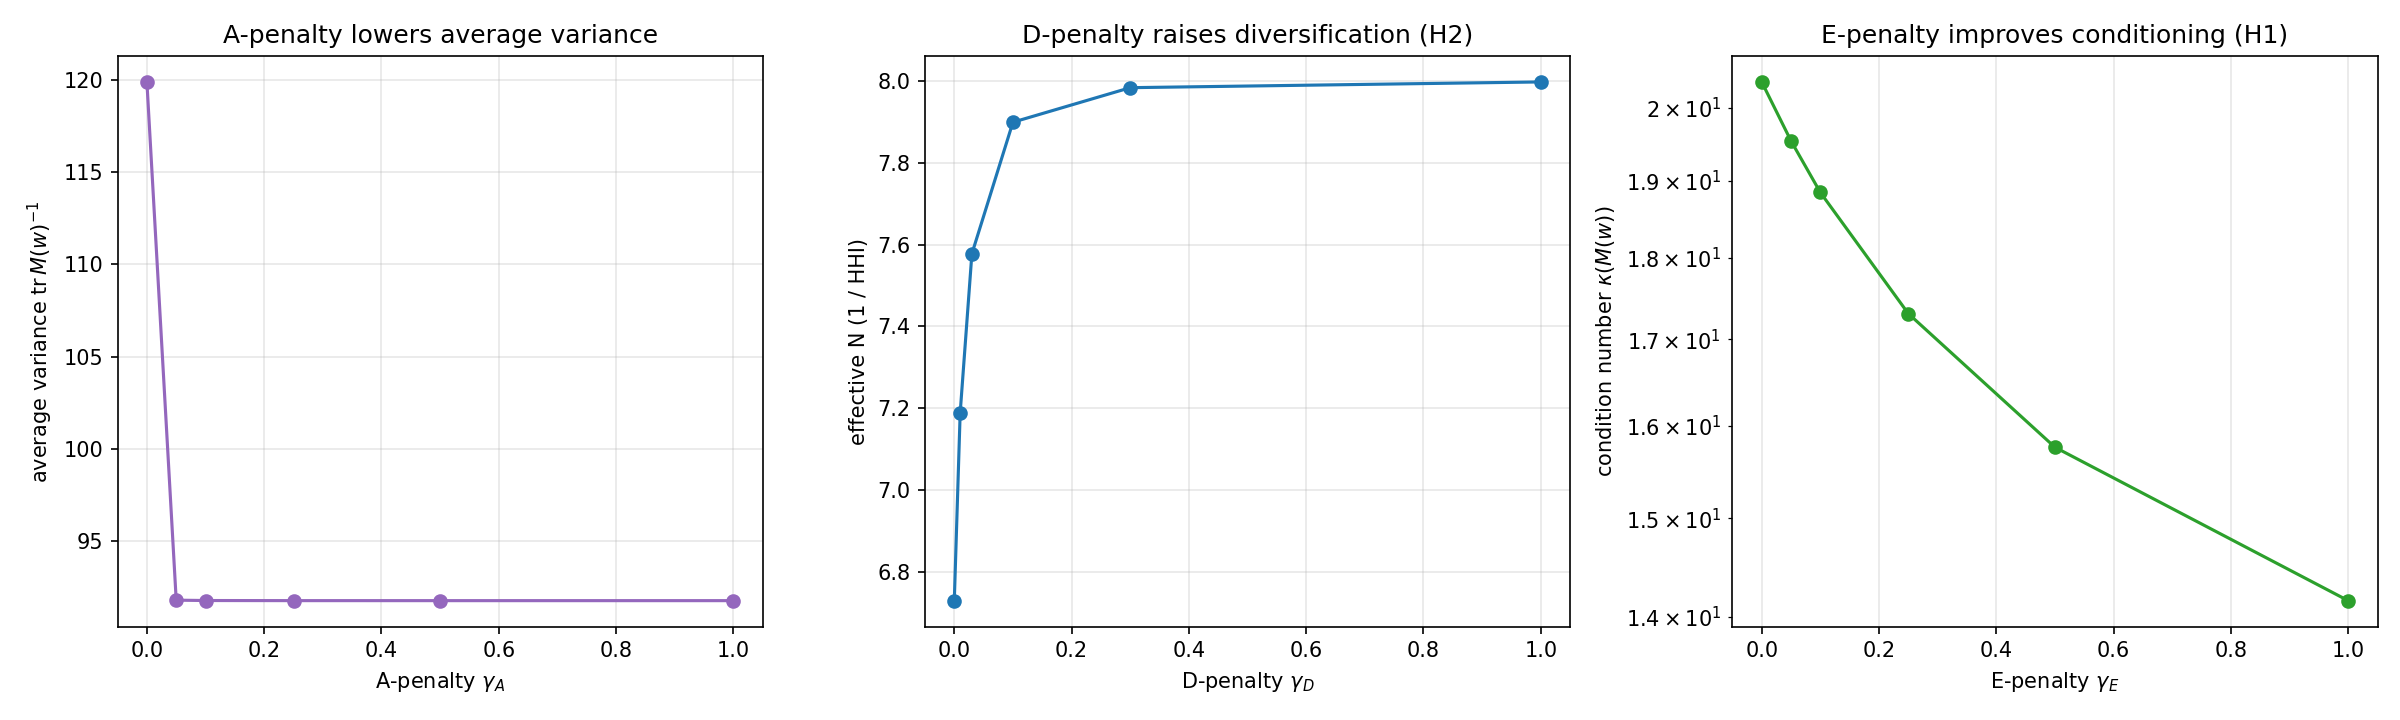
\includegraphics[width=\textwidth]{week6_design_penalty_sweep.png}
  \caption{Criterion sweeps (long-only, synthetic). Each design penalty improves
    its own target quantity: A lowers average estimation variance, D raises
    diversification, E improves worst-case conditioning.}
  \label{fig:sweep}
\end{figure}

\subsection{High-dimensional simulation ($N/T\to1$)}
We next stress the estimation problem directly. On a factor data-generating
process (low-rank signal plus idiosyncratic noise) we fix the estimation window
$T=120$ days and grow the universe $N\in\{15,40,80,110\}$, so the concentration
ratio $q=N/T$ rises from $0.125$ to $0.917$. As $q\to1$ the sample covariance
degrades sharply (Figure~\ref{fig:nt}, left panel of the estimator-error figure),
and the effect on the portfolios is stark. Table~\ref{tab:nt} reports the extreme
case $q=0.917$.

\begin{table}[h]
\centering
\caption{High-dimensional sweep at $q=N/T=0.917$ ($N=110$, $T=120$), factor DGP,
  averaged over seeds. Turnover and effective $N$ are the stability/diversification
  readouts.}
\label{tab:nt}
\begin{tabular}{lrrrr}
\toprule
\textbf{Strategy} & \textbf{Sharpe} & \textbf{OOS vol} & \textbf{Turnover} & \textbf{Eff.\ $N$} \\
\midrule
Equal weight            & 4.51 & 0.0347 & 0.000 & 110.0 \\
Markowitz (sample)      & 0.62 & 0.0551 & 3.401 & 8.3 \\
Ridge                   & \textbf{7.35} & \textbf{0.0169} & 0.084 & 101.6 \\
Shrinkage (Ledoit--Wolf)& 6.25 & 0.0186 & 0.402 & 65.5 \\
Proposed (D+E+ridge)    & 4.69 & 0.0327 & \textbf{0.0015} & \textbf{110.0} \\
\bottomrule
\end{tabular}
\end{table}

The sample-covariance Markowitz portfolio collapses (turnover $3.4$, effective
$N\approx8$, Sharpe $0.6$), while both the shrinkage and the design-regularized
portfolios remain stable. We report this honestly: as $q\to1$ the design penalty
wins decisively on \emph{turnover and diversification} (turnover $0.0015$ versus
$0.084$ for ridge, near-maximal breadth), but plain ridge attains the best raw
out-of-sample volatility. The design criteria and ridge are complementary rather
than competing---a point we return to in the discussion. A companion noise sweep
(fixing $N=30$, $T=120$ and fattening the tails via Student-$t$ innovations with
$\mathrm{df}\in\{3,5,10\}$) shows the same qualitative picture: the structured
methods hold their turnover and breadth as tails get heavy, while the raw
Markowitz weights become progressively more erratic.

\begin{figure}[h]
  \centering
  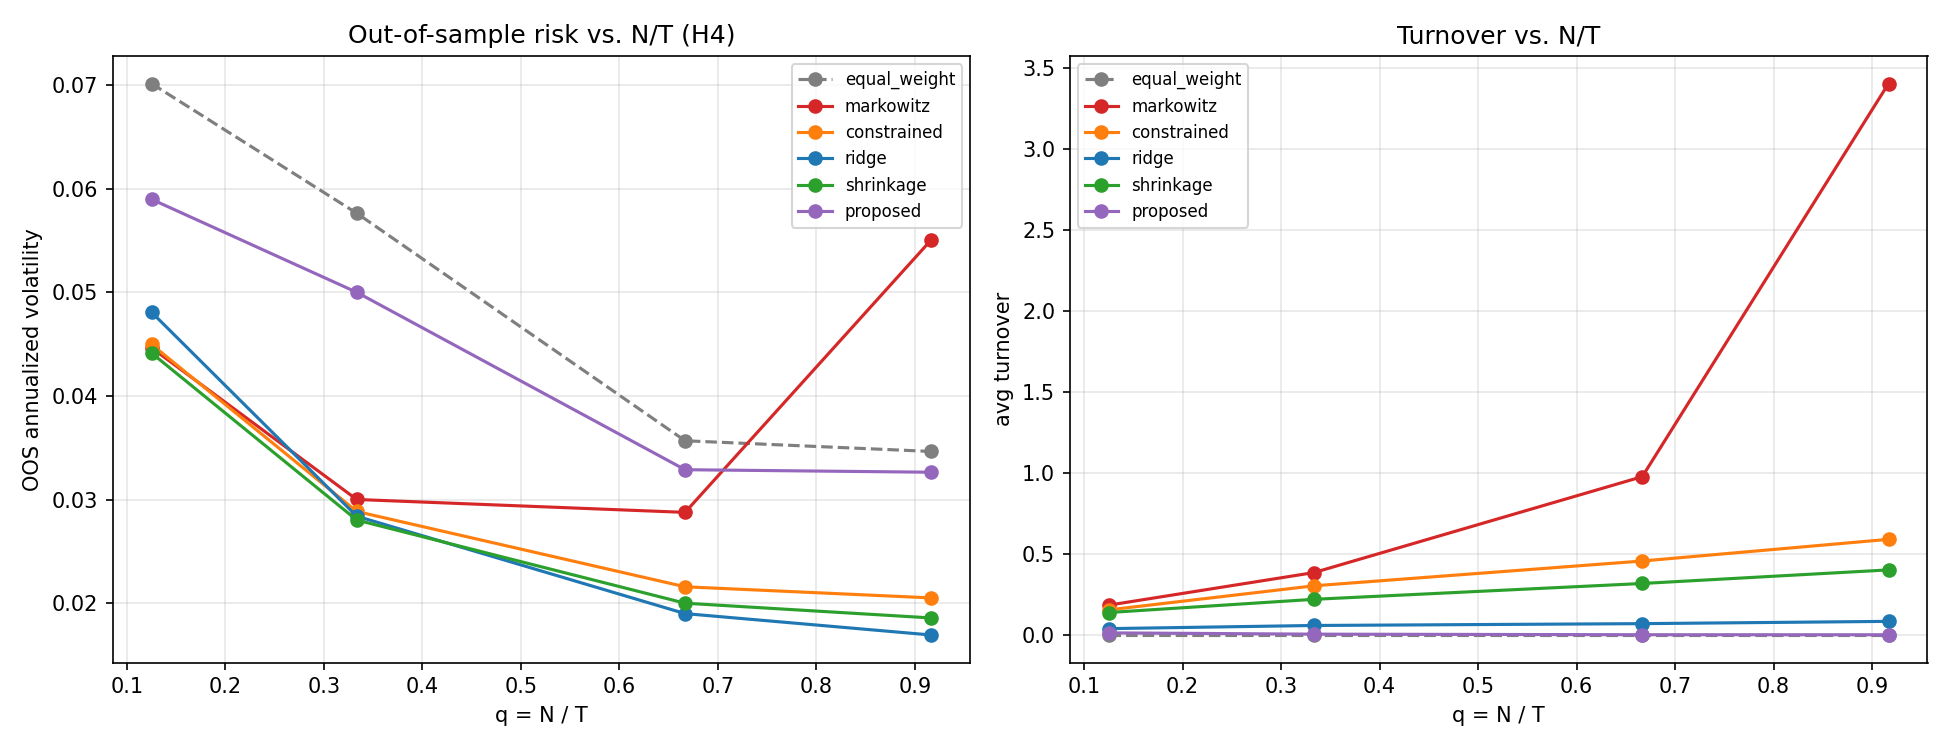
\includegraphics[width=\textwidth]{week7_method_vs_nt.png}
  \caption{High-dimensional behavior vs.\ concentration ratio $q=N/T$ (factor
    DGP). Left: out-of-sample volatility; right: average turnover. The sample
    Markowitz portfolio deteriorates as $q\to1$; the structured methods stay
    stable, with the design-regularized portfolio lowest on turnover.}
  \label{fig:nt}
\end{figure}

% =====================================================================
\section{Applications: real sector-ETF data}
% =====================================================================
We evaluate on a real universe of $11$ US sector ETFs (XLB, XLC, XLE, XLF, XLI,
XLK, XLP, XLRE, XLU, XLV, XLY), daily data from July 2018 to the present
($\approx2000$ observations). Using a rolling backtest with a $252$-day (one-year)
estimation window, monthly rebalancing, and out-of-sample holding, we compare six
strategies: equal weight, sample Markowitz (GMV), a constrained (capped) GMV,
ridge-GMV, Ledoit--Wolf shrinkage GMV, and the proposed design-regularized
portfolio. Table~\ref{tab:real} and Figures~\ref{fig:realmetrics}--\ref{fig:realeq}
report the panel.

\begin{table}[h]
\centering
\caption{Real sector-ETF backtest (2018--present, 252-day window, monthly
  rebalance, $84$ rebalances). Lower turnover and higher effective $N$ are
  better; ``Proposed'' is ridge $+$ D $+$ E with a $30\%$ cap.}
\label{tab:real}
\begin{tabular}{lrrrrr}
\toprule
\textbf{Strategy} & \textbf{Sharpe} & \textbf{OOS vol} & \textbf{Turnover} & \textbf{Eff.\ $N$} & \textbf{Max DD} \\
\midrule
Equal weight             & \textbf{0.751} & 0.1875 & 0.000 & 11.00 & $-0.363$ \\
Markowitz (sample)       & 0.483 & 0.1573 & 0.423 & 1.68 & $-0.338$ \\
Constrained GMV          & 0.651 & 0.1632 & 0.116 & 4.18 & $-0.332$ \\
Ridge GMV                & 0.655 & 0.1734 & 0.063 & 8.67 & $-0.357$ \\
Shrinkage GMV            & 0.528 & 0.1555 & 0.311 & 2.19 & $-0.343$ \\
Proposed (D+E+ridge)     & 0.710 & 0.1766 & \textbf{0.038} & \textbf{9.30} & $-0.355$ \\
\bottomrule
\end{tabular}
\end{table}

Reading the numbers honestly:
\begin{itemize}[leftmargin=1.4em,itemsep=0.2em]
  \item The raw sample Markowitz portfolio is the worst risk-adjusted performer
    (Sharpe $0.48$), concentrates in fewer than two effective names, and churns
    heavily (turnover $0.42$). This is the instability the paper is about.
  \item The \textbf{proposed} portfolio recovers almost all of the equal-weight
    risk-adjusted return (Sharpe $0.71$ vs $0.75$) while cutting turnover roughly
    \textbf{tenfold} versus sample Markowitz ($0.038$ vs $0.423$) and raising
    effective breadth from $1.7$ to $9.3$ names. It dominates every other
    \emph{optimized} strategy on the stability-for-return trade-off.
  \item Ridge alone already helps (turnover $0.063$, effective $N=8.7$); the
    design penalties push turnover lower still and breadth higher, at a small cost
    in out-of-sample volatility---consistent with the synthetic sweeps.
\end{itemize}

\begin{figure}[h]
  \centering
  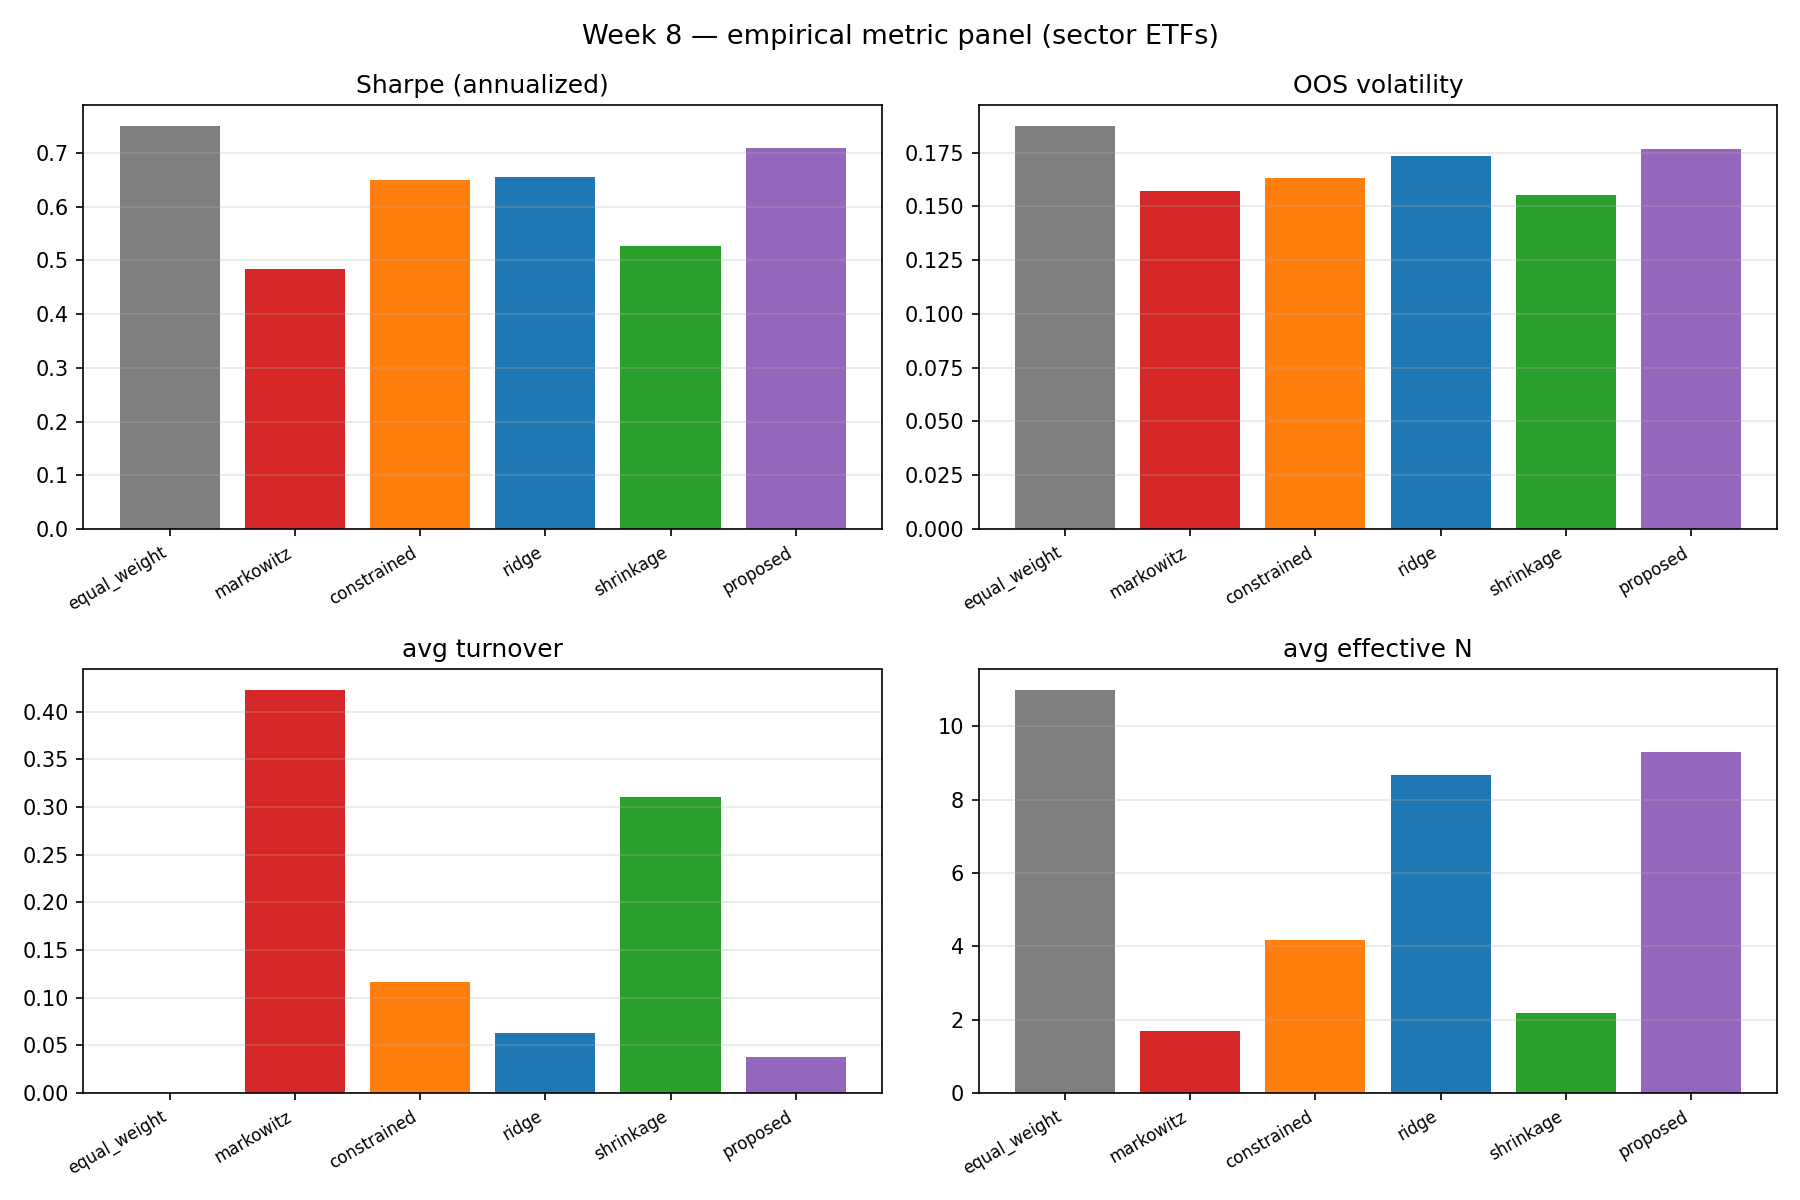
\includegraphics[width=\textwidth]{week8_metrics.png}
  \caption{Real sector-ETF metric panel: Sharpe, out-of-sample volatility,
    turnover, and effective $N$ by strategy. The proposed portfolio pairs
    equal-weight-like breadth with the lowest turnover among optimized methods.}
  \label{fig:realmetrics}
\end{figure}

\begin{figure}[h]
  \centering
  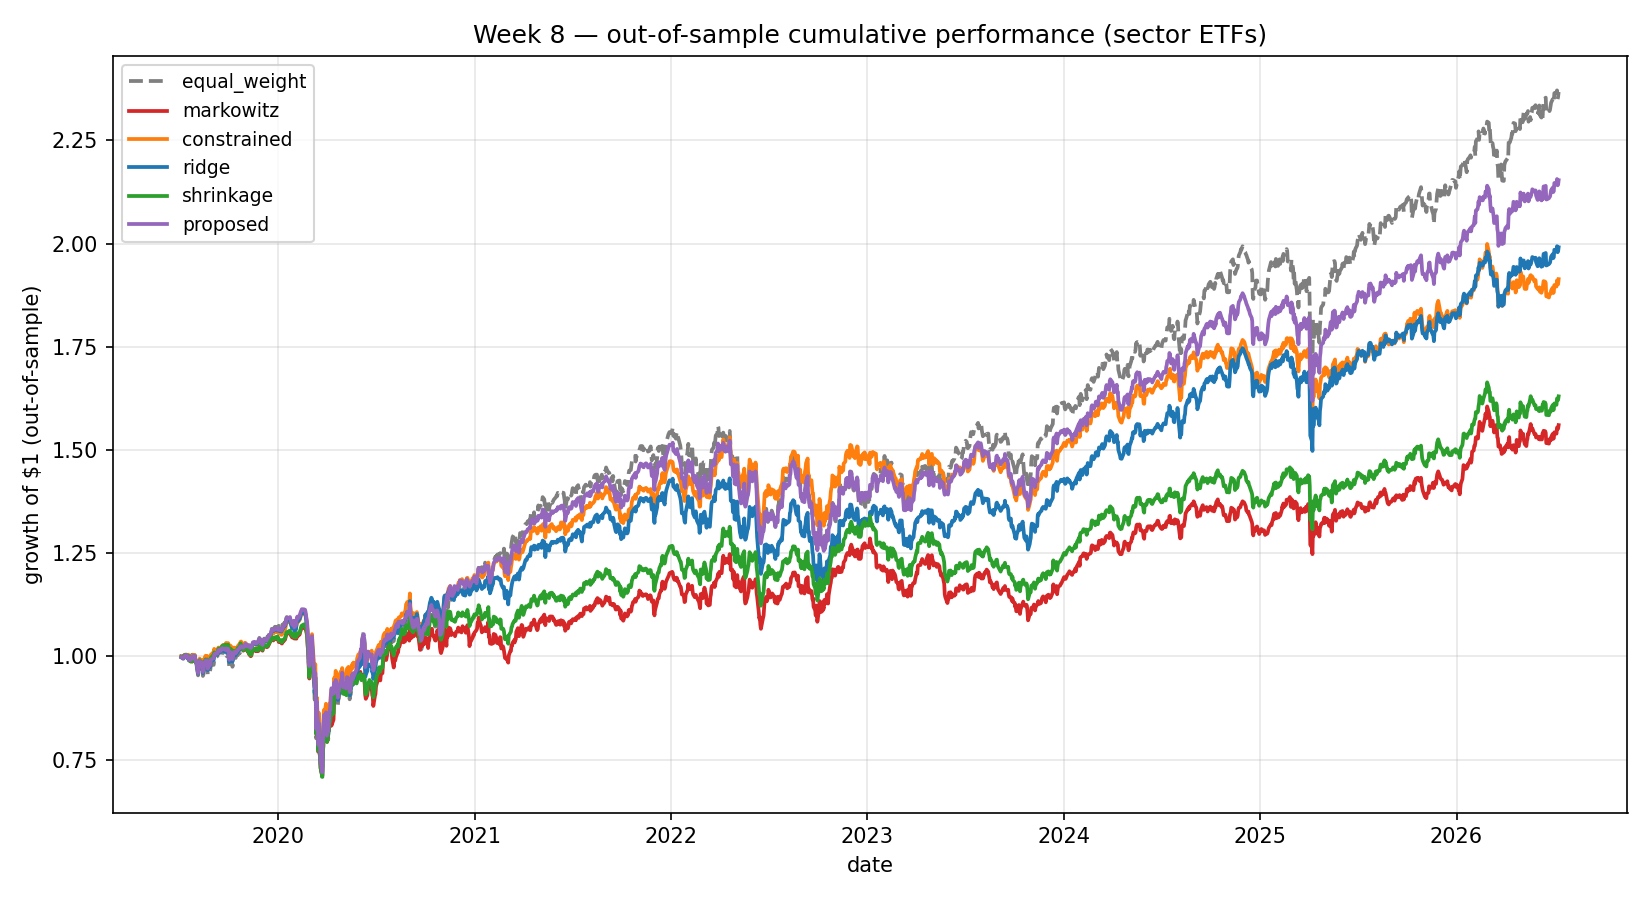
\includegraphics[width=0.82\textwidth]{week8_equity_curves.png}
  \caption{Out-of-sample cumulative growth of \$1 on the sector-ETF universe.}
  \label{fig:realeq}
\end{figure}

\paragraph{Transaction costs.} Because turnover translates directly into trading
cost, the turnover reduction is economically meaningful: under a linear cost model
the net-of-cost Sharpe ranking favors the low-turnover design-regularized
portfolio increasingly as the cost per unit turnover rises, whereas the raw
Markowitz portfolio's high turnover erodes its (already weak) gross performance.

\paragraph{Crisis vs.\ calm (preliminary).} Splitting the sample into stressed and
calm sub-periods gives a mixed but interpretable read on the E-criterion: in the
calm regime the robust (E-tilted) variant improves risk-adjusted return relative
to GMV, while in the crisis regime its realized volatility is comparable to
GMV's. The worst-case payoff of E is expected to be clearest under sharper,
out-of-sample stress; we flag this as the main direction for further empirical
work rather than an established result.

% =====================================================================
\section{Discussion}
% =====================================================================
\paragraph{When each criterion is useful.} The three criteria are not
substitutes; they target different properties, and the empirics bear this out:
\begin{itemize}[leftmargin=1.4em,itemsep=0.2em]
  \item \textbf{D (diversification)} is the most broadly useful as a stabilizer:
    it raises effective breadth and lowers turnover at little cost, and it is the
    cheapest to reason about (a log-barrier toward $1/N$).
  \item \textbf{E (robustness)} is the criterion to reach for when worst-case
    conditioning or robustness to a misspecified risk model matters; its benefits
    are clearest under stress and in ill-conditioned, high-$N$ regimes.
  \item \textbf{A (average variance)} regularizes the weights but trades
    \emph{portfolio} variance for \emph{estimation} variance; it is best viewed as
    a shrinkage device rather than a risk minimizer, and should be used with that
    caveat in mind.
\end{itemize}

\paragraph{Trade-offs and limitations.} The design penalties buy stability and
diversification, generally at a small cost in raw out-of-sample volatility versus
plain ridge---so the honest framing is that design regularization is
\emph{complementary} to ridge/shrinkage, adding turnover and breadth control on
top of spectral conditioning. The bridge is exact only at the matrix/criterion
level (information is linear in $\w$; risk is quadratic), the E-term is nonsmooth
where $\lammin$ is repeated, and the factor loadings $B$ must themselves be
estimated. The current experiments use the precision-metric ($V=\Sighat^{-1/2}$)
default; substituting explicitly estimated loadings (Fama--French or statistical
factors) into $\M=B^\top\diag(\w)B$ is the immediate next step and the cleanest
test of the factor interpretation of Section~\ref{sec:vi}.

\paragraph{Summary.} We have proposed a single convex optimizer that unifies
Markowitz risk, ridge regularization, and A/D/E design penalties, given the
design terms a genuine factor-regression meaning, established the theory
(convexity, gradients, KKT, uniqueness, exact reductions), and shown on synthetic,
high-dimensional, and real data that the design criteria each control a distinct,
named property of the portfolio---delivering, in particular, an order-of-magnitude
turnover reduction and a large gain in diversification at competitive
risk-adjusted return.

\bibliographystyle{plain}
\bibliography{refs}

\end{document}
